% Options for packages loaded elsewhere
\PassOptionsToPackage{unicode}{hyperref}
\PassOptionsToPackage{hyphens}{url}
\PassOptionsToPackage{dvipsnames,svgnames,x11names}{xcolor}
%
\documentclass[
  letterpaper,
  DIV=11,
  numbers=noendperiod]{scrartcl}

\usepackage{amsmath,amssymb}
\usepackage{iftex}
\ifPDFTeX
  \usepackage[T1]{fontenc}
  \usepackage[utf8]{inputenc}
  \usepackage{textcomp} % provide euro and other symbols
\else % if luatex or xetex
  \usepackage{unicode-math}
  \defaultfontfeatures{Scale=MatchLowercase}
  \defaultfontfeatures[\rmfamily]{Ligatures=TeX,Scale=1}
\fi
\usepackage{lmodern}
\ifPDFTeX\else  
    % xetex/luatex font selection
  \setmainfont[]{Atkinson Hyperlegible}
  \setsansfont[]{Atkinson Hyperlegible}
  \setmonofont[]{Fira Code}
\fi
% Use upquote if available, for straight quotes in verbatim environments
\IfFileExists{upquote.sty}{\usepackage{upquote}}{}
\IfFileExists{microtype.sty}{% use microtype if available
  \usepackage[]{microtype}
  \UseMicrotypeSet[protrusion]{basicmath} % disable protrusion for tt fonts
}{}
\makeatletter
\@ifundefined{KOMAClassName}{% if non-KOMA class
  \IfFileExists{parskip.sty}{%
    \usepackage{parskip}
  }{% else
    \setlength{\parindent}{0pt}
    \setlength{\parskip}{6pt plus 2pt minus 1pt}}
}{% if KOMA class
  \KOMAoptions{parskip=half}}
\makeatother
\usepackage{xcolor}
\setlength{\emergencystretch}{3em} % prevent overfull lines
\setcounter{secnumdepth}{-\maxdimen} % remove section numbering
% Make \paragraph and \subparagraph free-standing
\ifx\paragraph\undefined\else
  \let\oldparagraph\paragraph
  \renewcommand{\paragraph}[1]{\oldparagraph{#1}\mbox{}}
\fi
\ifx\subparagraph\undefined\else
  \let\oldsubparagraph\subparagraph
  \renewcommand{\subparagraph}[1]{\oldsubparagraph{#1}\mbox{}}
\fi


\providecommand{\tightlist}{%
  \setlength{\itemsep}{0pt}\setlength{\parskip}{0pt}}\usepackage{longtable,booktabs,array}
\usepackage{calc} % for calculating minipage widths
% Correct order of tables after \paragraph or \subparagraph
\usepackage{etoolbox}
\makeatletter
\patchcmd\longtable{\par}{\if@noskipsec\mbox{}\fi\par}{}{}
\makeatother
% Allow footnotes in longtable head/foot
\IfFileExists{footnotehyper.sty}{\usepackage{footnotehyper}}{\usepackage{footnote}}
\makesavenoteenv{longtable}
\usepackage{graphicx}
\makeatletter
\def\maxwidth{\ifdim\Gin@nat@width>\linewidth\linewidth\else\Gin@nat@width\fi}
\def\maxheight{\ifdim\Gin@nat@height>\textheight\textheight\else\Gin@nat@height\fi}
\makeatother
% Scale images if necessary, so that they will not overflow the page
% margins by default, and it is still possible to overwrite the defaults
% using explicit options in \includegraphics[width, height, ...]{}
\setkeys{Gin}{width=\maxwidth,height=\maxheight,keepaspectratio}
% Set default figure placement to htbp
\makeatletter
\def\fps@figure{htbp}
\makeatother

\usepackage{fancyhdr}
\pagestyle{fancy}
\fancyfoot[C]{\thepage}
\renewcommand{\headrulewidth}{0.4pt}
\renewcommand{\footrulewidth}{0.4pt}
\KOMAoption{captions}{tableheading}
\makeatletter
\@ifpackageloaded{caption}{}{\usepackage{caption}}
\AtBeginDocument{%
\ifdefined\contentsname
  \renewcommand*\contentsname{Table of contents}
\else
  \newcommand\contentsname{Table of contents}
\fi
\ifdefined\listfigurename
  \renewcommand*\listfigurename{List of Figures}
\else
  \newcommand\listfigurename{List of Figures}
\fi
\ifdefined\listtablename
  \renewcommand*\listtablename{List of Tables}
\else
  \newcommand\listtablename{List of Tables}
\fi
\ifdefined\figurename
  \renewcommand*\figurename{Figure}
\else
  \newcommand\figurename{Figure}
\fi
\ifdefined\tablename
  \renewcommand*\tablename{Table}
\else
  \newcommand\tablename{Table}
\fi
}
\@ifpackageloaded{float}{}{\usepackage{float}}
\floatstyle{ruled}
\@ifundefined{c@chapter}{\newfloat{codelisting}{h}{lop}}{\newfloat{codelisting}{h}{lop}[chapter]}
\floatname{codelisting}{Listing}
\newcommand*\listoflistings{\listof{codelisting}{List of Listings}}
\makeatother
\makeatletter
\makeatother
\makeatletter
\@ifpackageloaded{caption}{}{\usepackage{caption}}
\@ifpackageloaded{subcaption}{}{\usepackage{subcaption}}
\makeatother
\ifLuaTeX
  \usepackage{selnolig}  % disable illegal ligatures
\fi
\usepackage{bookmark}

\IfFileExists{xurl.sty}{\usepackage{xurl}}{} % add URL line breaks if available
\urlstyle{same} % disable monospaced font for URLs
\hypersetup{
  pdftitle={Lab 6 Worksheet},
  colorlinks=true,
  linkcolor={blue},
  filecolor={Maroon},
  citecolor={Blue},
  urlcolor={Blue},
  pdfcreator={LaTeX via pandoc}}

\title{\textbf{Lab 6 Worksheet}}
\usepackage{etoolbox}
\makeatletter
\providecommand{\subtitle}[1]{% add subtitle to \maketitle
  \apptocmd{\@title}{\par {\large #1 \par}}{}{}
}
\makeatother
\subtitle{Getting started with Qualtrics \& Gorilla}
\author{}
\date{}

\begin{document}
\maketitle

\raggedright

\section{Starting Developing Your
Studies}\label{starting-developing-your-studies}

\subsection{By the end of the session, you will
have:}\label{by-the-end-of-the-session-you-will-have}

\begin{itemize}
\tightlist
\item
  Worked together in your groups to determine next steps in your
  studies; specifically, materials that are shared, and those that are
  individual to you. This will allow you to divide and conquer!
\item
  Registered for a Goldsmiths Qualtrics account.
\item
  Opened the `Mini-Dissertation Qualtrics Template' in your account.
\item
  Started editing the template according to your needs.
\item
  Considered randomizing blocks in your survey to avoid order effects.
\item
  Set up scoring to save you time computing scores.
\item
  If your study requires complex stimulus presentation or reaction
  times, you'll want to use Gorilla. A brief overview of valuable
  resources is available.
\end{itemize}

Work with your group to identify which elements of your study (measures,
questionnaires, tasks) are shared and which are individual. This will
allow you to start considering how to combine your energies to best
effect in developing materials.

Most, if not all, of you, will use Qualtrics. There are some useful
tools and tips to help you get up and running. Import the
Mini-Dissertation Template and get to work building your study. For more
complex tasks, Gorilla will be what you need.

Gordon's Top Tip: Time spent preparing your materials really pays off --
in terms of time, data quality, and confidence!

\subsection{Working Out How to Start Developing Your
Study}\label{working-out-how-to-start-developing-your-study}

\begin{enumerate}
\def\labelenumi{\arabic{enumi}.}
\item
  \textbf{Moving towards your individual research question:} In your
  groups, and with your Critical Proposals in mind, discuss your
  projects. Do you all still agree on your original research question or
  how you thought you'd explore it? Have your ideas developed in any
  way? List your preferred IVs, DVs, and methodologies and compare
  notes. Look out for similarities and differences.

  It is normal that your approaches or interests may diverge a little as
  a result of your critical evaluations. This is great. If not, that's
  fine too. The design of your individual Mini-Dissertation needs to be
  slightly different from your collaborators, so you can pursue your
  interests if they differ somewhat.

  Exploring different personality traits is a nice way to find
  distinctive IVs. If you are presenting stimulus materials, you could
  present different types, classes, or categories. An exploration of
  memory may include familiar or unfamiliar words, short or long words,
  or focus on another type of stimulus, such as numbers or shapes,
  different presentation durations, or recall delays. Or you could use
  different DVs, such as accuracy/error rate, or reaction time, or
  confidence; all interesting. If you are looking at life-outcomes as a
  DV (as many of you are), these can vary by domain (e.g.~work or
  home-life) or how you quantify them; how do you quantify success or
  happiness or health? It may initially seem quite tricky to see how
  this might work, but your lab tutor is on hand to help!
\item
  \textbf{Sharing the workload:} Following on from the question above,
  is there a `central' task, measure, or stimulus-set in your project
  that potentially requires more effort to find or build? Does some
  aspect of your project involve the selection or creation of stimulus
  material?

  This might be a good thing to develop as a group, allowing you to make
  it as effective as possible. This is likely the core of your methods
  section and worth making fabulous. You can then duplicate this
  component and break into smaller groups to tailor it and collect the
  data if you need to or want to. But by working together as much as
  possible, you can refine this component and make it as accurate and
  impressive as possible with relative ease.
\end{enumerate}

\subsection{Opening a Goldsmiths Qualtrics
Account}\label{opening-a-goldsmiths-qualtrics-account}

\begin{enumerate}
\def\labelenumi{\arabic{enumi}.}
\item
  Please go to this link:
  \href{https://goldpsych.eu.qualtrics.com/}{Goldsmiths Qualtrics}
\item
  Use your college email address and password. To get the full
  functionality, you MUST use your college login.

  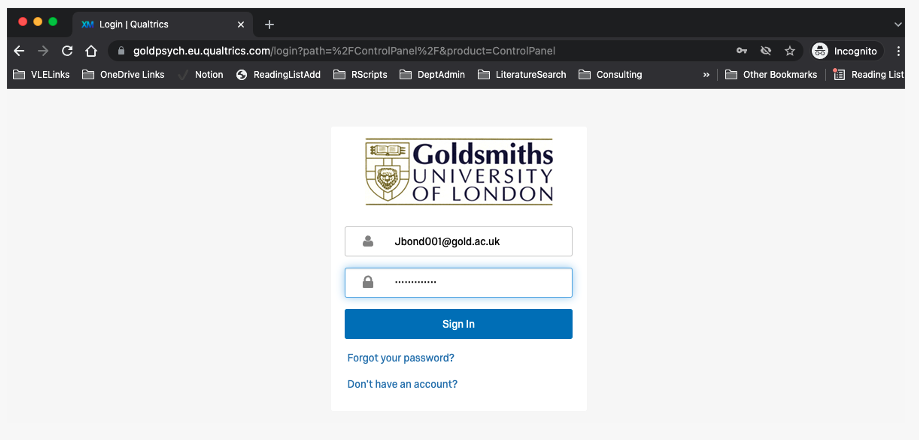
\includegraphics{images/Screenshot - Microsoft Word-10-11-000232.png}
\item
  If you accidentally set up a trial account, or use a different email,
  it can take 3 weeks to change. Follow these instructions on the VLE:
  \href{https://learn.gold.ac.uk/mod/url/view.php?id=1410095}{VLE
  Instructions}
\item
  You will know if you have been successful if, when you log in, the URL
  starts with goldpsych.eu.qualtrics.com.
\end{enumerate}

\subsection{Importing the Mini-Dissertation
Template}\label{importing-the-mini-dissertation-template}

\begin{enumerate}
\def\labelenumi{\arabic{enumi}.}
\item
  Download the Mini-Dissertation Qualtrics Template
  \href{https://learn.gold.ac.uk/mod/resource/view.php?id=1410096}{HERE}
  or from the VLE page.
\item
  It will be a .qsf file, native to Qualtrics, and will only open in
  Qualtrics.
\item
  To use the template, on the Homepage, click on `Create a new project',
  select `Survey', and `Get started'.

  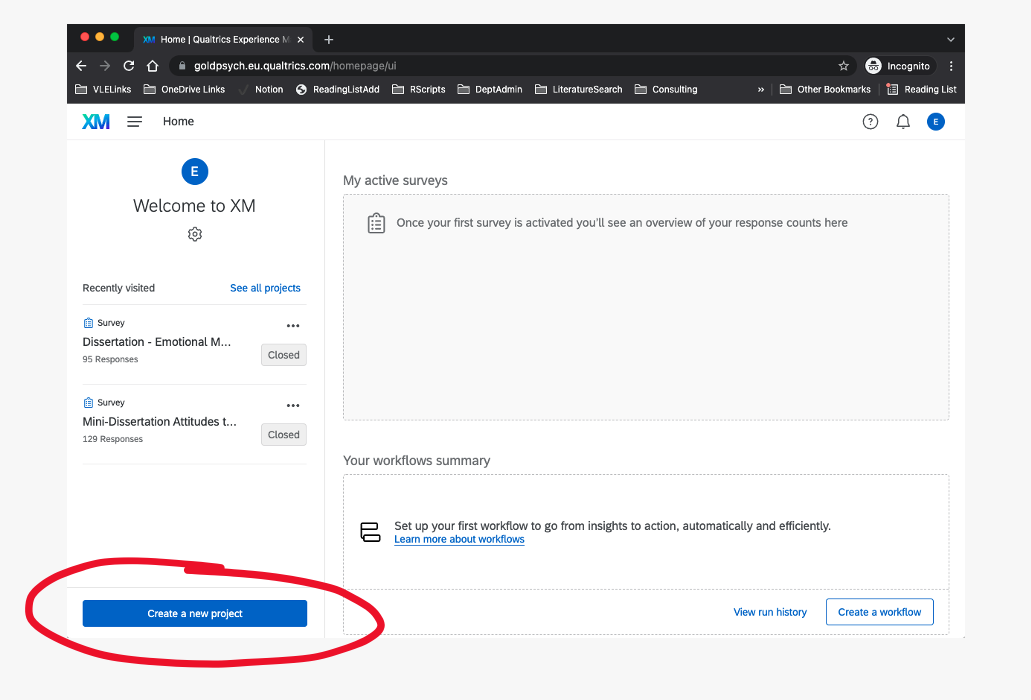
\includegraphics{images/Screenshot - Microsoft Word-10-11-000234.png}
\item
  Give your project a preliminary name (this can be changed later) and
  choose `Import a QSF file' from the `How you want to start' dropdown.

  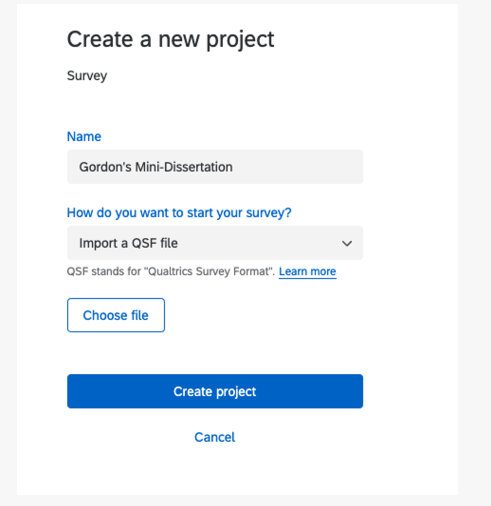
\includegraphics{images/Screenshot - Microsoft Word-10-11-000238.png}
\item
  Find the .qsf file you downloaded earlier using the `Choose file'
  finder and then click `Create project'.
\item
  You will likely be offered the option to `Take a tour' of the Survey
  Builder. It takes two minutes and shows you how to change settings and
  to edit questions.

  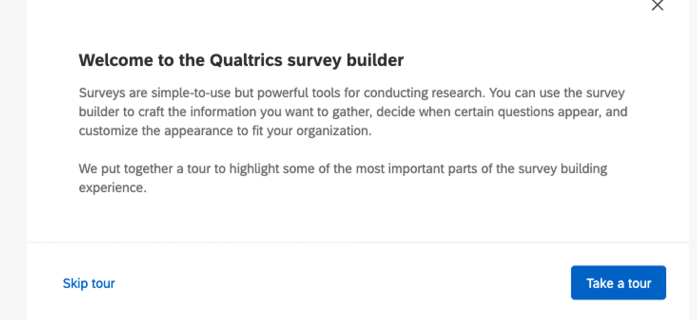
\includegraphics{images/Screenshot - Microsoft Word-10-11-000240.png}
\end{enumerate}

\subsection{The Template}\label{the-template}

Please notice that, over and above the survey questions, the template
includes four important elements; 1) an Information Sheet outlining the
study, 2) Informed Consent, 3) GDPR, and 4) a Debrief delivered at the
end of the survey.

You are required to submit copies of the information you supply in these
sections in word doc format with your Ethics Application for storage on
file. Simply copy the content in the relevant sections of your Qualtrics
survey into 4 separate word documents for submission.

NB: If you run an experiment in person (this year OR next), you will be
required to give each participant a hard copy of all of these documents
and retain a signed Consent Form for your records. The process of
developing these materials is valuable preparation - please be involved.

Once you've created your survey, you're ready to start building. This
page outlines how to add, delete, copy, and edit multiple questions in
the Survey tab to build your required functionality. The Qualtrics help
is extremely useful and gives extensive, easily-navigable help.

For example, you will want to add new questions into the body of the
survey, corresponding with demographic information or a psychometric
measure or questionnaire you have found.

\subsection{New Questions in your
Survey}\label{new-questions-in-your-survey}

This page is very useful to help select the best question type. There
are many types, but you will find Matrix Tables, Multiple Choice, and
Sliders particularly useful. You can present images, media and text by
using the Text/Graphic options and Rich Text Editor.

\begin{itemize}
\tightlist
\item
  \href{https://www.qualtrics.com/support/survey-platform/survey-module/editing-questions/creating-questions/?parent=p0030\#AddingNewQuestions}{Creating
  New Questions in Qualtrics}
\end{itemize}

Try to make the questions as easy to navigate as possible. Remember to
use page breaks to make the flow more enjoyable.

\begin{itemize}
\tightlist
\item
  \href{https://www.qualtrics.com/support/survey-platform/survey-module/editing-questions/add-page-break/?parent=p0030\#AddingPageBreaksManually}{Adding
  Page Breaks Manually}
\end{itemize}

You can use a Rich Content Editor to include more elaborate instructions
and adding media or graphics. You can also use hyperlinks to connect to
content on the web outside of your questionnaire. You might want to
include a downloadable file, such as a debrief form or pdf of some
information you think a participant may want to retain. This can be
managed via the Rich Content Editor. Making a participant feel like they
have learned something can be a powerful reward. Please be careful not
to break copyright by sharing materials you haven't produced yourself.
If you propose to include such materials, this should be included in
your Ethics Application.

\subsection{Important safety and ethics
considerations}\label{important-safety-and-ethics-considerations}

Please only use your Goldsmiths Email address when running research and
if you give your own details ALWAYS supply those of your Lab Tutor or
the Module Coordinator. This affords you some protection and allows us
to help deal with any questions.

It is important that you clearly outline recruitment strategies in your
ethic application (i.e.~how you propose to recruit and where you share
your task) and you must ONLY share an approved task.

\subsection{Block Options and
randomisation}\label{block-options-and-randomisation}

\begin{itemize}
\tightlist
\item
  \href{https://www.qualtrics.com/support/survey-platform/survey-module/block-options/block-options-overview/?parent=p00101}{Block
  Options and Randomization}
\end{itemize}

Sets of questions (or entire questionnaires) can be set up as `blocks'
within your survey. If you wish to randomize these blocks, you can,
meaning that you can randomly shuffle the sequence of presentation. This
is an important feature that you may wish to consider using. Obviously,
the information and informed consent will need to remain at the start
and the debrief needs to always be the last block presented.

In the `survey flow' area, you will see that you can view the blocks in
the survey and add a randomizer, that randomly delivers a selection of
blocks. Block 1 and 2 are identical in the template, but will be
presented in random order for each new participant.

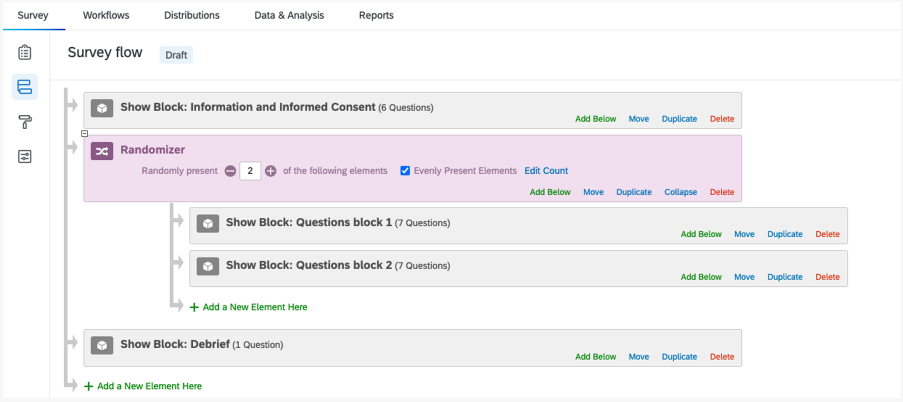
\includegraphics{images/Screenshot - Microsoft Word-10-11-000242.png}

\subsection{Recoding and Scoring (Massive time
savers!)}\label{recoding-and-scoring-massive-time-savers}

\subsubsection{Recode Values}\label{recode-values}

Once you have set up your survey, it is always a good idea to run a test
and export the data to make sure it is in the format that you require.
If you notice that the data are not in the format you would most easily
use, it may be that you could consider `recoding' the values to make it
easier to use.

\begin{itemize}
\tightlist
\item
  \href{https://www.qualtrics.com/support/survey-platform/survey-module/question-options/recode-values/}{Recode
  Values in Qualtrics}
\end{itemize}

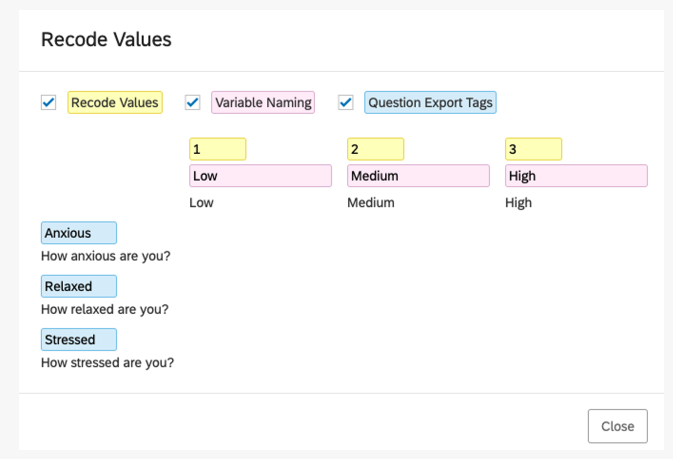
\includegraphics{images/Screenshot - Microsoft Word-10-11-000244.png}

\subsubsection{Scoring questionnaires}\label{scoring-questionnaires}

Scoring can save you LOTS of time, by automatically scoring your
questionnaires or subscales of your questionnaires. Consider using this
if your measure generates a total score or you are planning on
calculating an average etc. It is perfectly easy to calculate these in
excel, but it can be done automatically with a little care and
preparation.

\begin{itemize}
\tightlist
\item
  \href{https://www.qualtrics.com/support/survey-platform/survey-module/survey-tools/scoring/\#Introduction}{Scoring
  in Qualtrics}
\end{itemize}

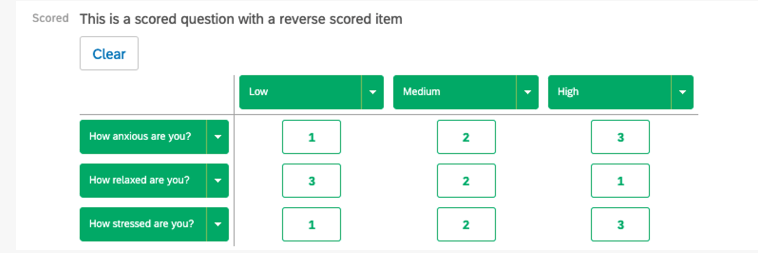
\includegraphics{images/Screenshot - Microsoft Word-10-11-000246.png}

\subsection{Previewing your survey}\label{previewing-your-survey}

If you want to see how a question (or entire survey) looks, use the
preview functionality. It will allow you to see what the participant
will see -- both on a computer and on a mobile device.

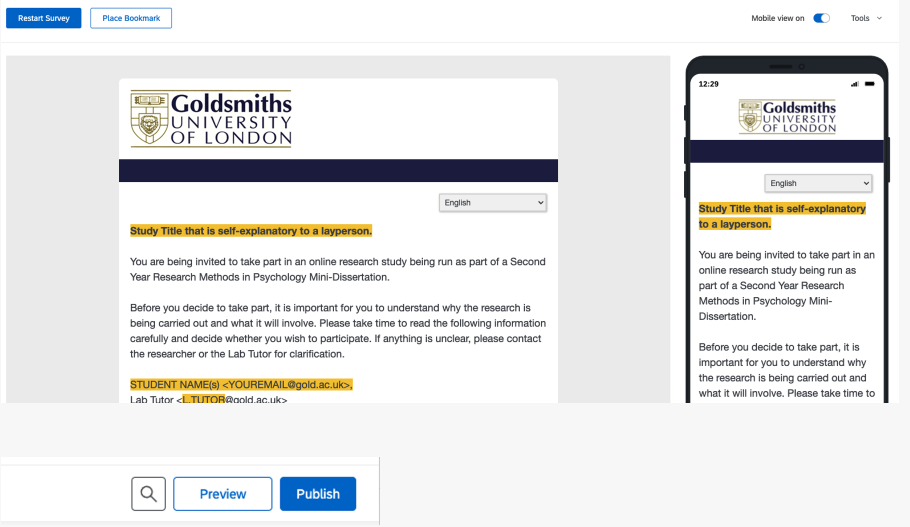
\includegraphics{images/Screenshot - Microsoft Word-10-11-000248.png}

\subsection{Data Export}\label{data-export}

It is highly recommended that you test how the data will be exported
from your survey, so that you can perfect how you label your questions
and how you recode or score your variables. To run a quick `data test'
do the following.

Click Publish and label the versions `Data Test' and click `Publish'
again.

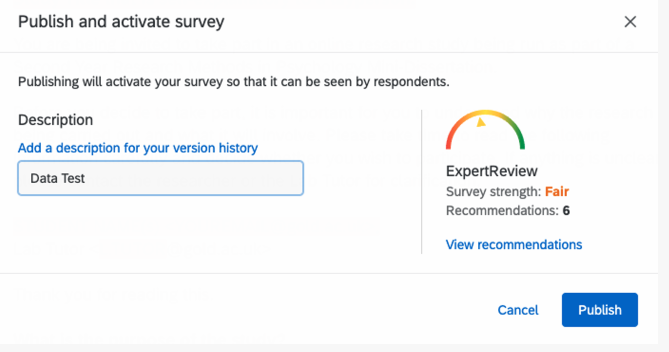
\includegraphics{images/Screenshot - Microsoft Word-10-11-000250.png}

Under `Distributions' select `Anonymous link' (which is how you will
share your study with participants usually. You can of course produce a
QR code or use Bit.ly to shorten the link to make it more attractive.
Think about the best way to recruit for your study.

Copy the link to your browser and run through the study.

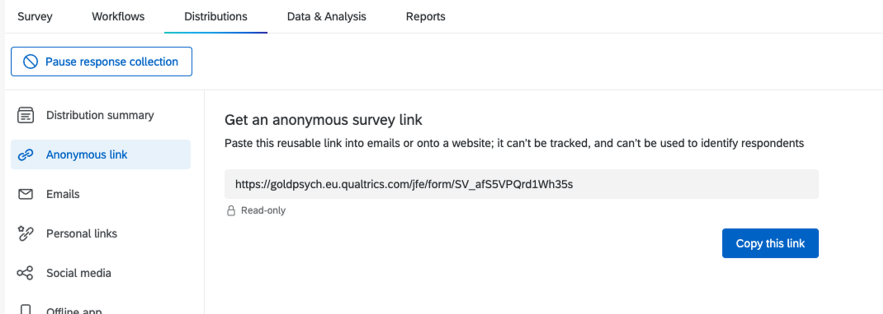
\includegraphics{images/Screenshot - Microsoft Word-10-11-000252.png}

Export Data from this menu to a range of useful formats.

\begin{figure}[H]

{\centering 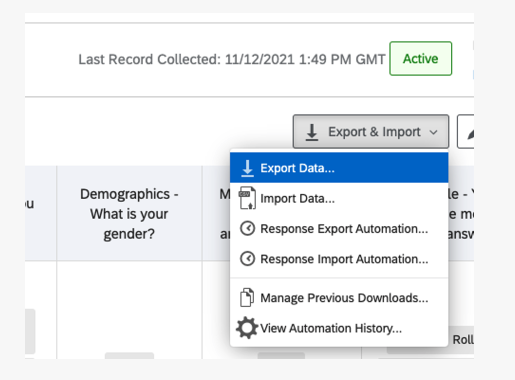
\includegraphics{images/Screenshot - Microsoft Word-10-11-000254.png}

}

\end{figure}%

In Term 2 we will be looking at the data and how to clean it. The most
important thing I would advise you to do is to name your blocks and
questions clearly, so that this is reflected in the dataset that you
download. If you don't know which question is which, you could come
unstuck.

\subsection{Collaborate your survey with
colleagues}\label{collaborate-your-survey-with-colleagues}

If you wish to share your survey with your group and work on it
together, you can `Collaborate' the project. It's like using a shared
document. You can monitor versions in case you make a mistake, but
remember to `Publish' if you want to over-write any changes you make!
You can find this in the `Tools' menu and you will need to use your
colleagues' Goldsmiths email addresses AND they will need to have a
Goldsmiths Qualtrics account too.

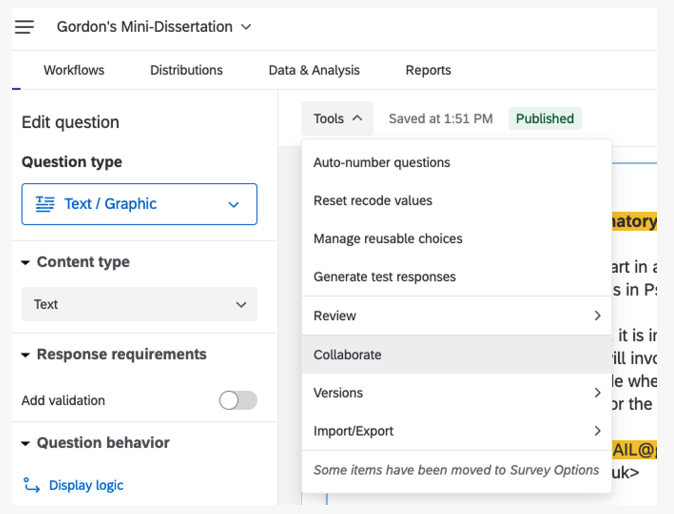
\includegraphics{images/Screenshot - Microsoft Word-10-11-000258.png}

For More Information the Qualtrics website includes comprehensive and
easy-to-follow help documentation as mentioned above. Tutorials,
webinars and detailed directions are available via Qualtrics' extensive
online resource, Qualtrics Support. \url{www.qualtrics.com/support}

For fast, individualized support over chat, email or a scheduled phone
call, please consider using the Support Center. We pay for the services
here, but they are based in the US:
\url{www.qualtrics.com/support-center}

For fast, individualized support over chat, email or a scheduled phone
call, please consider using the Support Center. We pay for the services
here, but they are based in the US:
\url{www.qualtrics.com/support-center}

\section{\texorpdfstring{\textbf{Gorilla.sc experimental
platform}}{Gorilla.sc experimental platform}}\label{gorilla.sc-experimental-platform}

Some of you may be keen to program a task, such as a Stroop Task or a
Go/No-Go task. For anything requiring complex presentation of stimuli or
data recording accuracies or reaction times, Gorilla would be the most
suitable platform to employ. Review some of the tasks they have in their
`Samples' collection ready for cloning!
\url{https://app.gorilla.sc/support/samples}

\textbf{Getting your Gorilla account if you are a new user to the
software please follow the below guidance:}

Please go the Gorilla webpage (\url{https://gorilla.sc/login}), if you
don't already have an account create a new one, at the bottom of STEP 3
- finish, you should find a box called + My institution already has a
subscription. Please click on this box (please see an image below for
ease) and enter the enrolment code: \textbf{PsychGold}

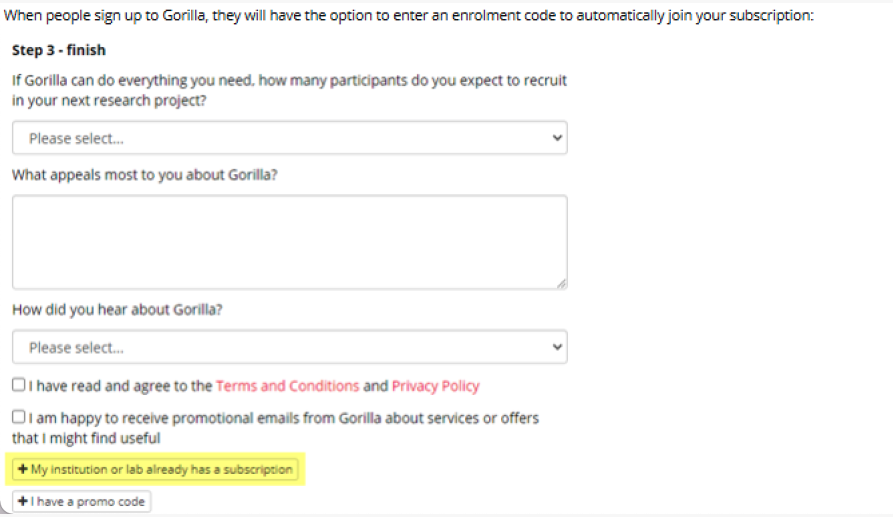
\includegraphics{images/Screenshot - Microsoft Word-10-11-000260.png}

\subsection{\texorpdfstring{\textbf{Support pages and other guides to
get you
started}}{Support pages and other guides to get you started}}\label{support-pages-and-other-guides-to-get-you-started}

There is a fantastic set of resources available to new users

\url{https://support.gorilla.sc/support/}

With a `Getting Started Guide'
\url{https://support.gorilla.sc/support/walkthrough/getting-started}

And onboarding videos
\url{https://support.gorilla.sc/support/getstarted}

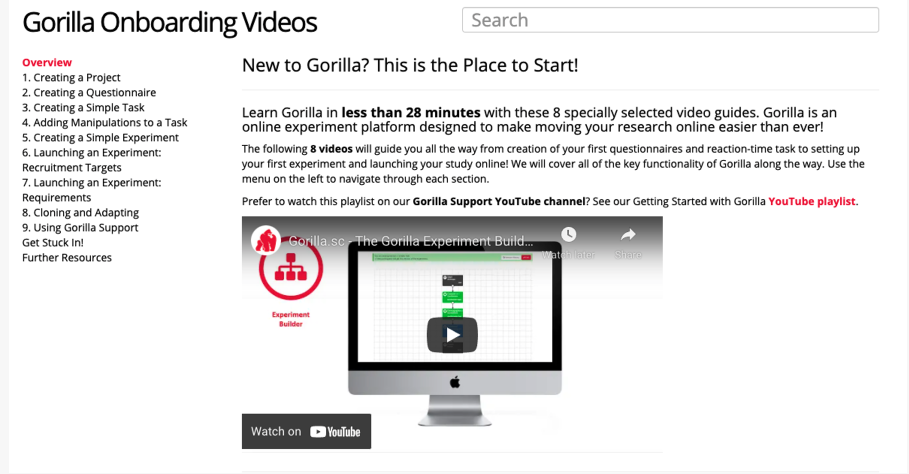
\includegraphics{images/Screenshot - Microsoft Word-10-11-000262.png}

\textbf{Gordon's Top Tip: Time spent preparing your materials really
pays off -- in terms of time, data quality and confidence!}

This is an exciting point in term. You've critically evaluated research
to inform your own approach to the topic. You've probably identified
useful measures and tasks to use in your studies. Now is the time to
start developing your studies for real.

Some of your studies may comprise questionnaire measures and other
demographic or participant details. Some may involve more complex
behavioural tasks. Even in person studies might benefit from using
Qualtrics or a computerised task.

Bear in mind that you need to have completed building these BEFORE you
apply for ethics later this term. Once your materials are approved, they
can't be changed. Now is the time to make them as effective as possible
in terms of the research question, but also as user-friendly as possible
-- for you AND the participants. The quality of these materials will
directly impact the quality of your data.

There will be some pragmatic decisions that you make, such as
identifying economical measures for variables of interest. A study that
is too time-consuming will be unattractive and you are required to
estimate how long a study takes to complete to participants before they
take part. Always consider the user experience. There is no requirement
that your study is long and complicated. This is a modest first research
study. There is no benefit to long and complicated!

And you should consider how user-friendly your materials are for
participants and experimenter alike. Try to make the materials you
employ appear professional and attractive. You will be submitting your
materials and they will be appraised for professionalism and
presentation. But thinking of yourself next term, the easier it is to
output your data and begin your analysis, the better.

Take the time to label your questions clearly and verify the data
outputs in an intelligible format. We will cover this in later labs, but
why not poke around in advance and ensure it's a smooth process! Take
the time to recode variables into output that you can use easily. And
use `Scoring' to give you automatically produced means, totals and
subscales wherever possible. It will save you time and worry in Term 2!

Simply put; being as confident in your materials as possible will save
you time and increase your confidence in the New Year (and Next Year!)

\textbf{Looking forward to Third Year: Data collection and management as
valuable skills}

You might think that something like Qualtrics isn't a hugely valuable
skill to learn. Well, in a high proportion of cases you'll use it next
year for your Final Year Dissertation, and being confident doing that is
worthwhile in itself.

But you'd be amazed how common it is nowadays to want to survey opinion
or attitudes. Imagine you are running a business and want to find out
what your customers think about your product. Imagine you are managing
an organization and need to understand how much time your employees
spend on unnecessarily difficult tasks, or how they rate you as a boss.

Asking questions using surveys is a quick way to generate important
insights, but not as easy as people think. Being able to design good
questions, and delivering them well, is a valuable skill.

And once you have lots of lovely data, being able to manage those data
well enough to allow you to extract the important insights hiding within
is something that very few people are able to do well\ldots{} You'll be
expert at such things.

I've already mentioned that Excel (or Numbers or Google Sheets) are
incredibly common tools you'll probably use on a regular basis in your
future lives. Contact lists, customer databases, financial results and
accounts, stock inventories, meta-data, Gannt charts and the list goes
on. We are training you in important skills here!

Being confident manipulating and presenting data -- Data Literacy - is
something you will likely wish to highlight on future CVs and you can
begin to develop those skills in your Mini-Dissertation, and refine and
perfect them next year. Being confident with data will allow you to
think bigger about your Final Year Dissertation than if you are worried
about this.

Many of you will be anxious about `statistics'. I'd hope, in due course,
that your experience this year will help to allay those fears. But I
believe the biggest anxiety students experience around `statistics'
isn't the statistics part of it at all. I believe that moving from raw
data to an analysis-ready dataset is the intimidating bit, not the few
button presses in SPSS. For this reason, we have oodles of support in
Term 2 around how to prepare, clean, and screen your data, so that you
can unleash all the SPSS skills you've been learning in Design \&
Analysis with zero stress.

Have a great week.



\end{document}
